\documentclass[12pt,a4paper]{article}
\synctex=1
\usepackage[utf8]{inputenc}
\usepackage[margin=1cm]{geometry}
\usepackage{graphicx}
%\usepackage{verbatim}
\usepackage{amsmath}
\usepackage{amsfonts}
\usepackage{amssymb}
\usepackage{listings}
\usepackage{enumitem}
\usepackage{textcomp}
\usepackage{courier}
\usepackage{libertine}
\usepackage{pgfornament}
\usepackage{eso-pic}
\usepackage[hangul]{kotex}
\linespread{1.3}

\title{
	\centering
	\pgfornament[width=12cm,color=teal]{84}\\
	\vspace{1cm}
	\fontsize{50}{50} \selectfont {정보통신 수학 및 실습\\Homework}\\
		\pgfornament[width=12cm,color=teal]{88}\\
	\vfill}
\author{
	\LARGE
	\begin{tabular}{rl}
		\hline
		학번 : & 2016110056\\ 
		학과 : & 불교학부 \\
		이름 : & 박승원\\
		날짜 : & \today\\
		\hline
	\end{tabular}\vspace{2cm}
	\\
\includegraphics[width=0.5\textwidth]{logo.jpg}
	}
\date{}


\begin{document}
\maketitle
\pagenumbering{gobble}
\noindent
\lstset{language=matlab, columns=flexible, tabsize=4, frame=shadowbox, showstringspaces=false, breaklines=true, upquote=true, basicstyle=\normalsize}

\renewcommand{\thesubsubsection}{\alph{subsubsection})}
\renewcommand{\thesubsection}{\arabic{subsection}.}
\newpage

\section*{Chapter 10 Homework}
\subsection{Find the Fourier series of the following functions. } 
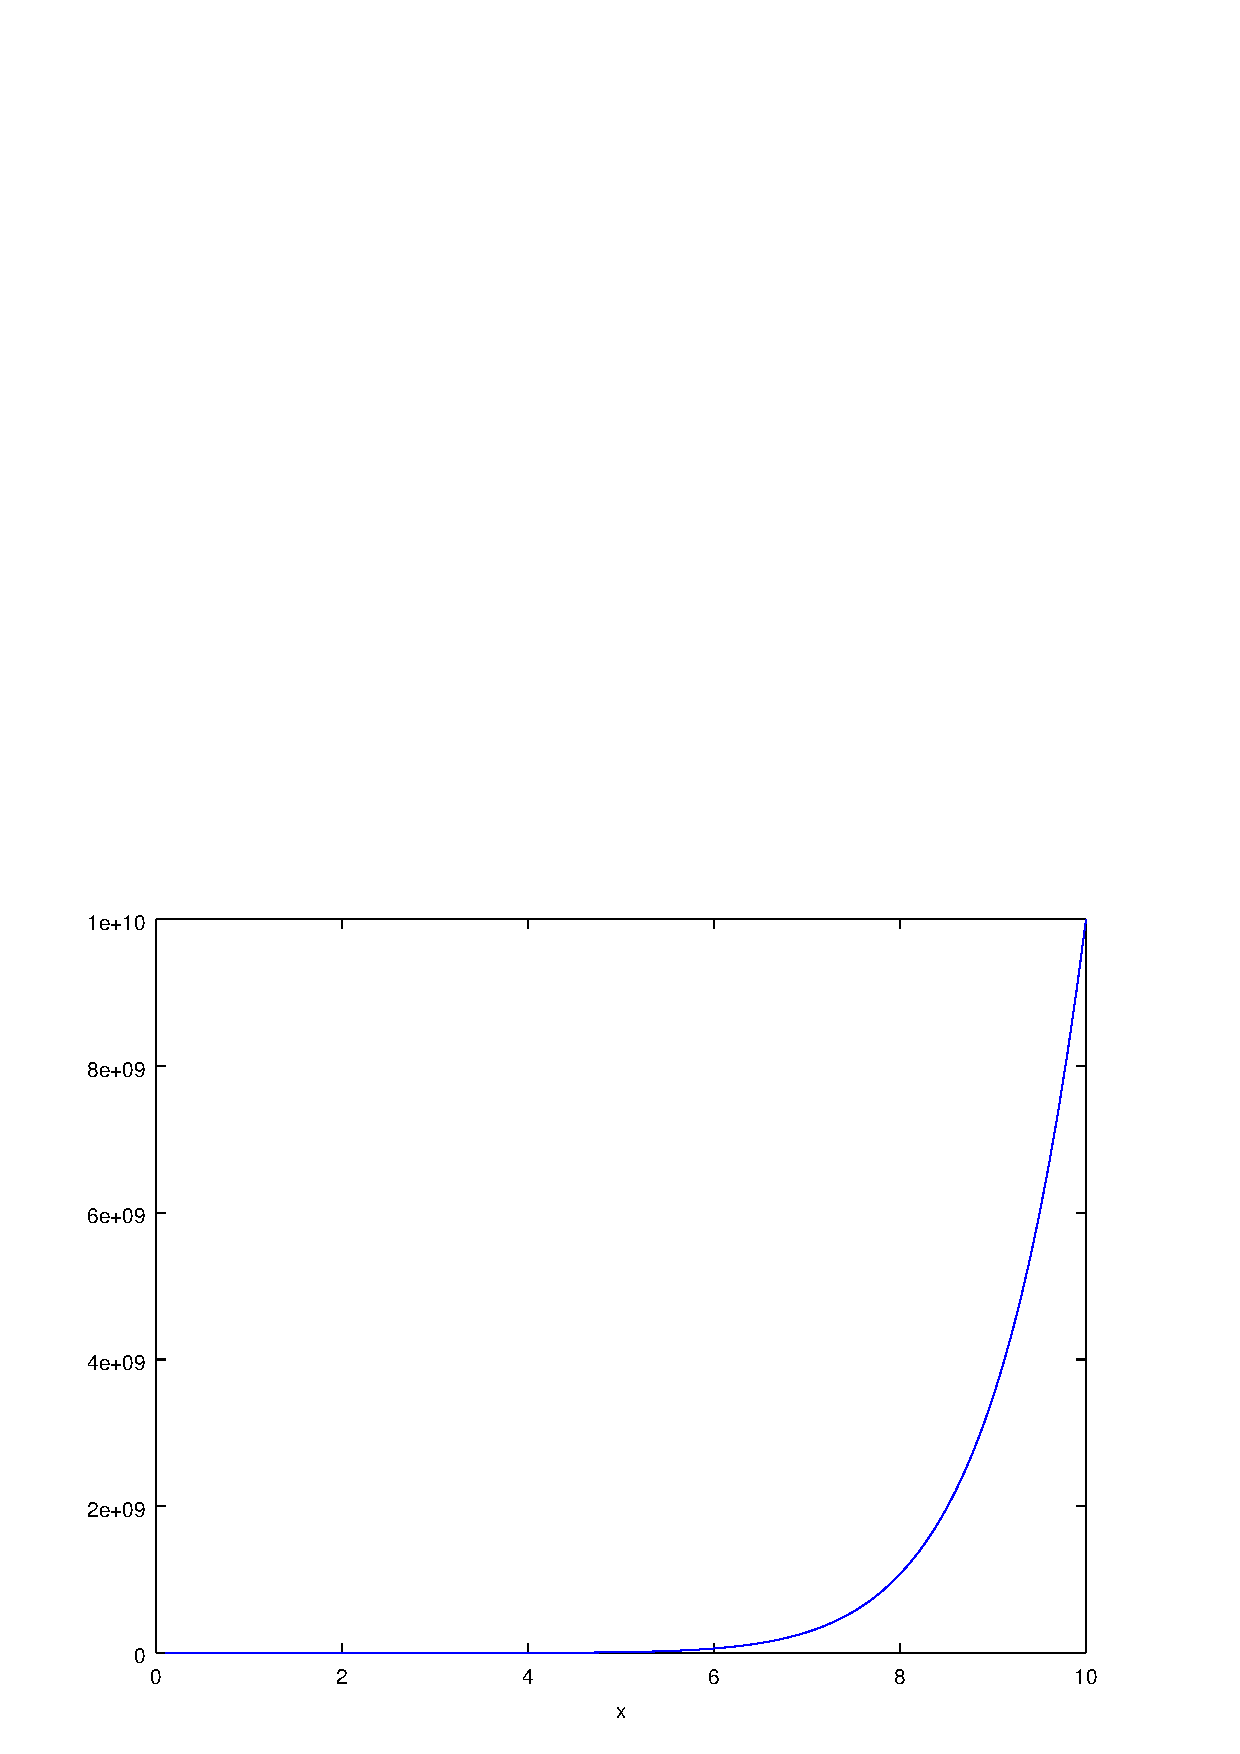
\includegraphics[width=\textwidth]{1.png}

even function 
\begin{gather*}
f(t) = a_0 + b_1 \cos t + b_2 \cos 2t + \cdots\\
a_0 = \int_{-\pi}^\pi f(t) dt = 0.2\\
b_n = \int_{-\pi}^\pi f(t)\cos(nt) dt
=\int_{-0.1}^{0.1}\cos(nt)dt
=\left[\frac{1}{n}\sin(nt)\right]_{-0.1}^{0.1}
=\frac{2}{n}\sin(0.1n) \\
\therefore f(t) = \sum_{k=1}^{n} 0.2 + \frac{2}{k}\sin(0.1k)
\end{gather*}
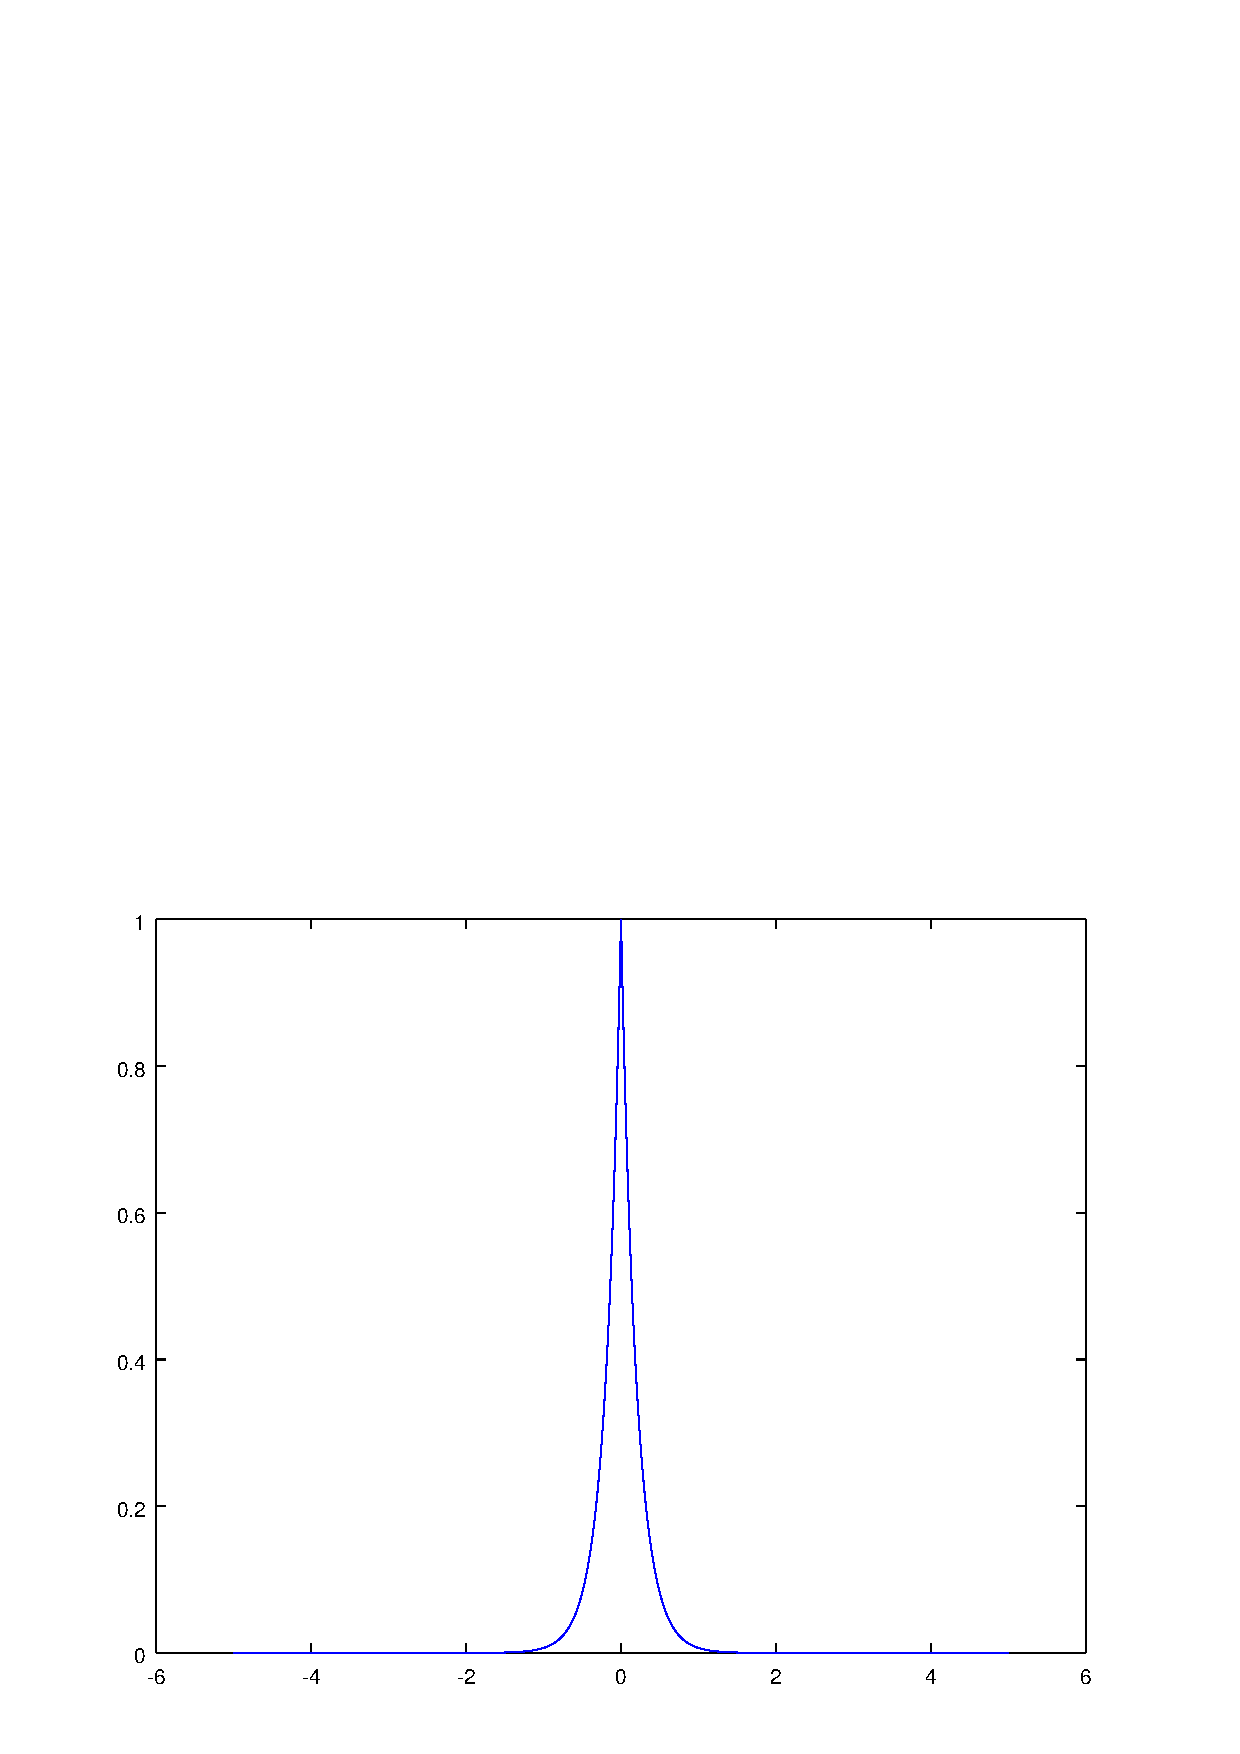
\includegraphics[width=\textwidth]{2.png}
\begin{gather*}
f(t) = a_0 + b_1 \cos \pi t + b_2 \cos 2\pi t+ \cdots\\
a_0 = \int_{-1}^1 f(t) = 0\\
b_n = \int_{-1}^{1}f(t)\cos(n\pi t)dt
=2(\int_0^{0.5}\cos(n\pi t)dt -\int_{0.5}^{1}\cos(n\pi t)dt)
=2(\left[\frac{1}{n\pi}\sin(n\pi t)\right]_0^{0.5} - \left[\frac{1}{n\pi}\sin(n\pi t)\right]_{0.5}^1)
=\frac{4}{n\pi}\\
\therefore f(t) = \sum_{k=1}^n \frac{4}{k\pi}\cos (k\pi t)
\end{gather*}
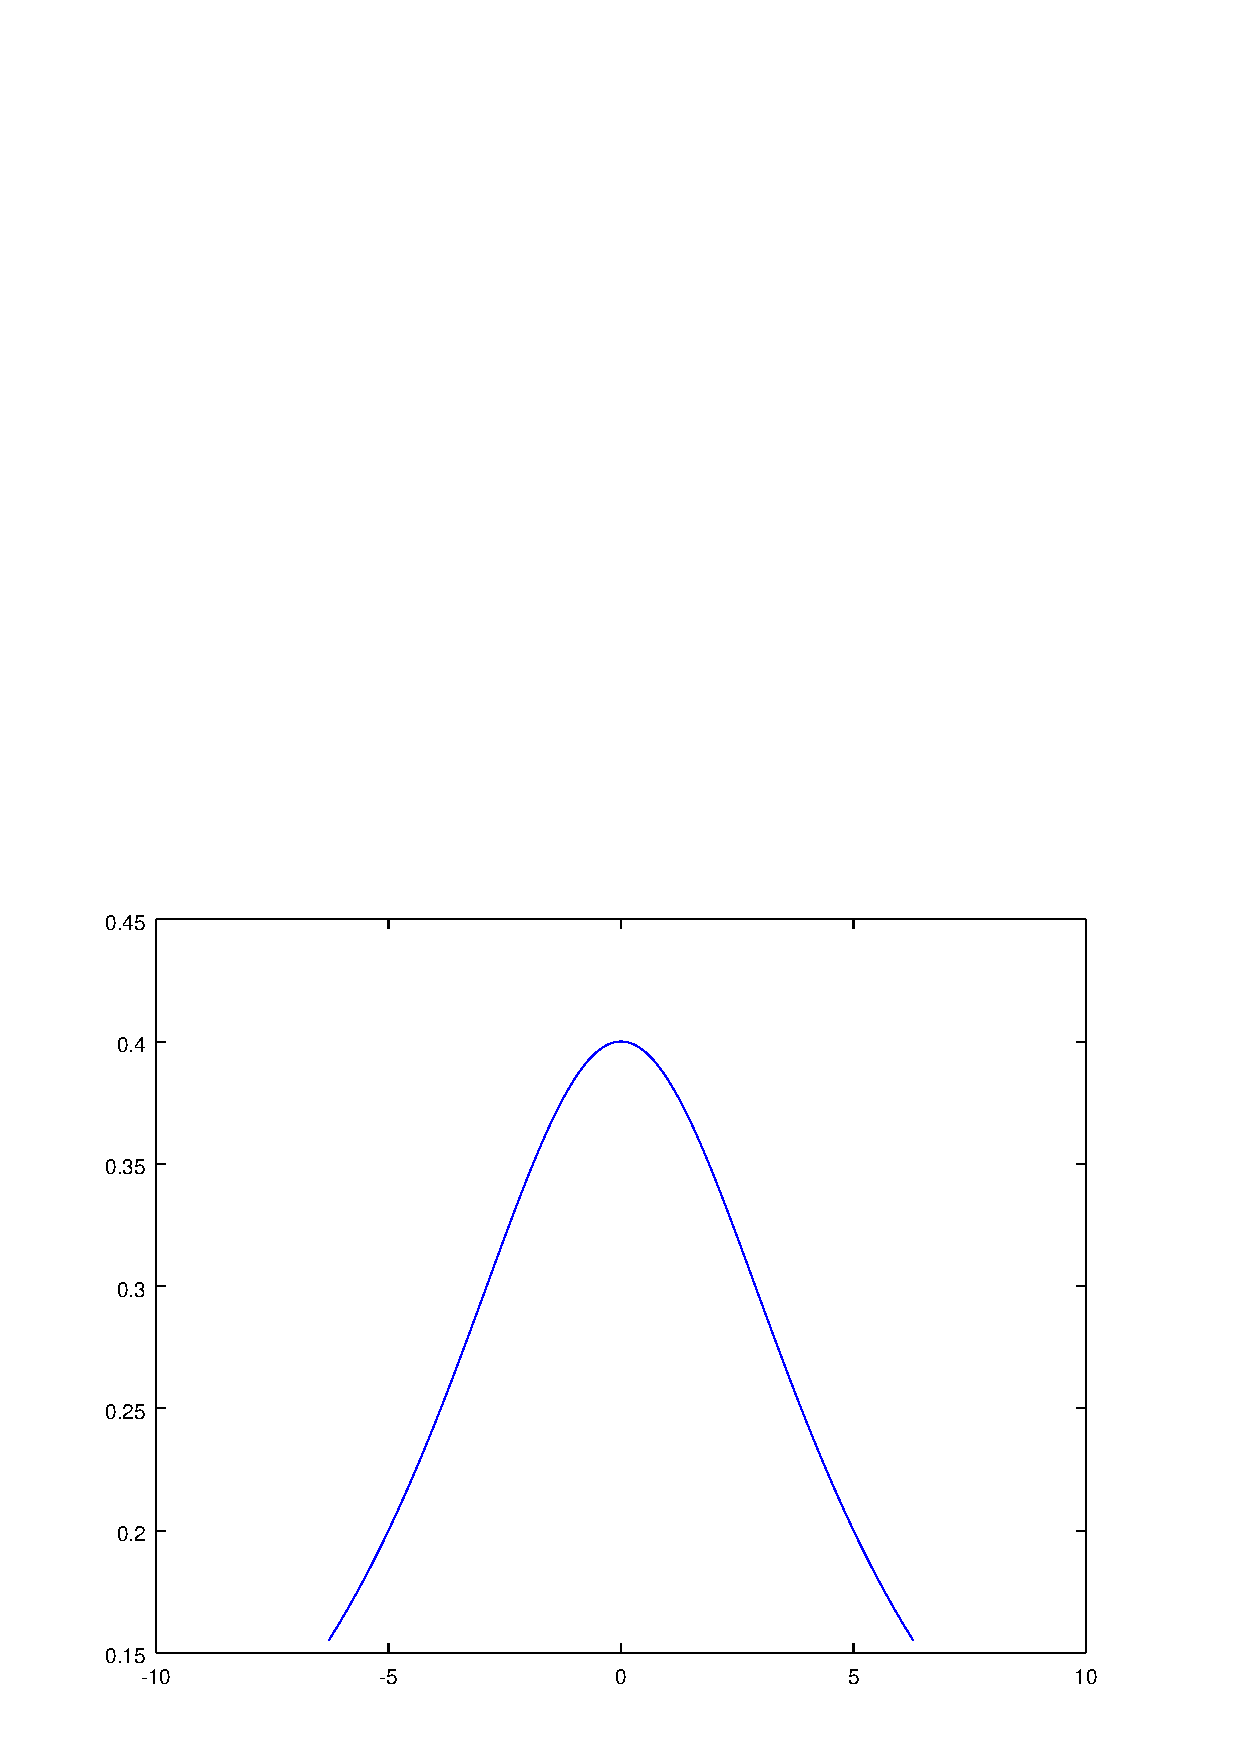
\includegraphics[width=\textwidth]{3.png}
\begin{gather*}
f(t) = a_0 + b_1 \sin 0.5t + b_2\sin t + b_3\sin 1.5t\cdots\\
a_0 = \int_{-2\pi}^{2\pi}f(t)dt = 0 \\
b_n = \int_{-2\pi}^{2\pi}f(t)\sin(0.5nt)dt
=4\int_0^\pi f(t)\sin(0.5nt)dt = -4\int_0^\pi t\sin(0.5nt)dt\\
\int uv' = uv - \int u'v\\
=-4(\left[t\cdot -\frac{2}{n}\cos\frac{nt}{2}\right]_0^\pi +\int_{0}^{\pi}\frac{2}{n}\cos\frac{nt}{2}dt)
=-4(\frac{-2t}{n}\cos(n\pi) + \left[\frac{4}{n^2}\cdot \sin\frac{nt}{2}\right]_0^\pi)
=-4(\frac{-2t}{n}\cos(\frac{n\pi}{2})+\frac{4}{n^2}\sin(\frac{n\pi}{2}))
\end{gather*}
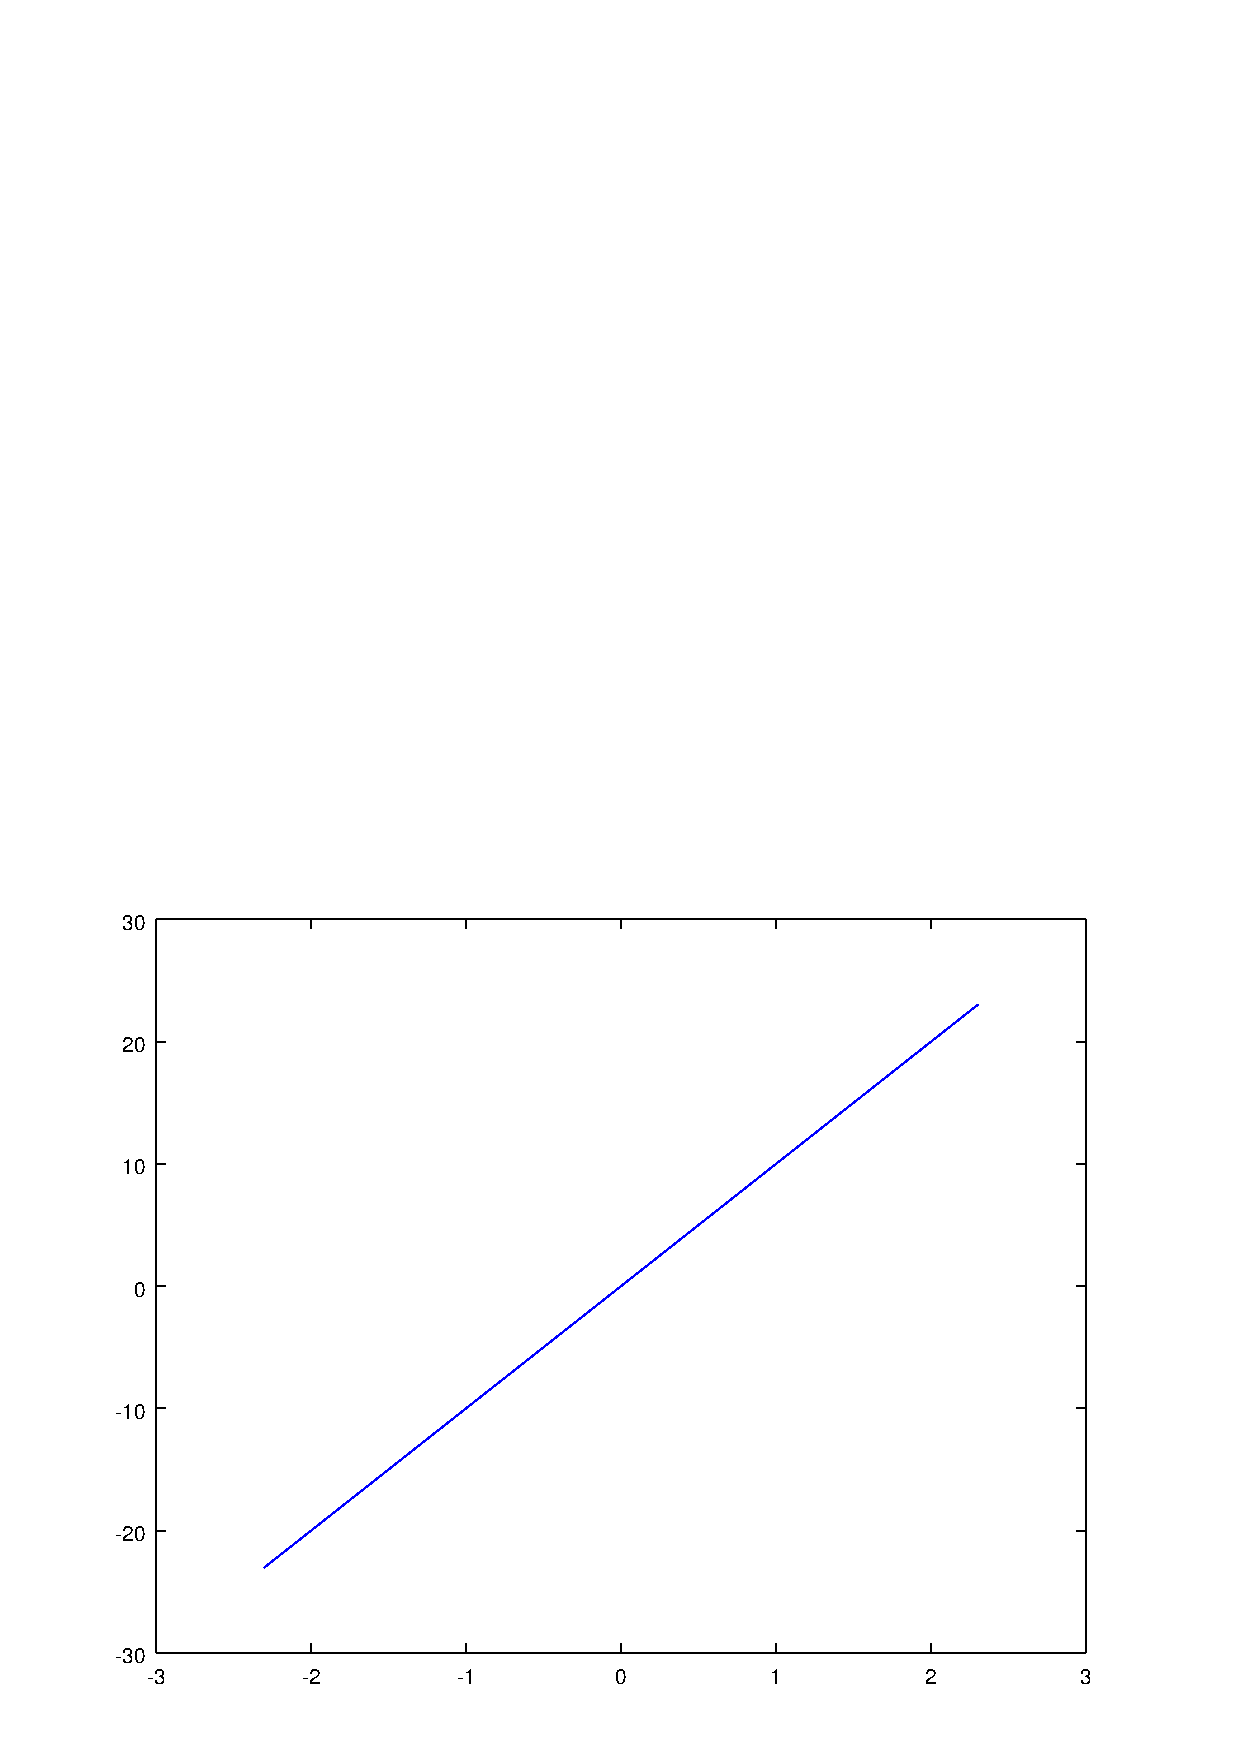
\includegraphics[width=0.5\textwidth]{4.png}
\begin{gather*}
f(t)=a_0 + b_1 e^{jt} + b_2 e^{2jt} + \cdots\\
a_0 = \int_{-\pi}^{\pi} f(t) dt
=\int_0^\pi \cos t dt = \left[\sin t\right]_0^\pi = 0\\
b_n = \int_{-\pi}^{\pi}f(t)e^{-jnt}dt
=\int_0^\pi \cos t e^{-jnt}dt
=\left[e^{-jnt}\sin t\right]_0^\pi -\int_0^\pi -jne^{-jnt}\sin t dt
=jn\int_0^\pi e^{-jnt}\sin t dt\\
=jn(\left[e^{-jnt}\cdot -\cos t\right]_0^\pi - \int_0^\pi jne^{-jnt}\cos t dt)\\
=jn((e^{-jn\pi} + 1) -n^2(\left[e^{-jnt}sint\right]_0^\pi)+\int_0^\pi -jne^{-jnt}\sin t dt)\\
b_n = jn(e^{-jn\pi} +1) -jnb_n)\\
b_n = jne^{-jn\pi} +jn + n^2b_n\\
\therefore b_n = \frac{jne^{-jn\pi}+jn}{1-n^2}
\end{gather*}
\end{document}
